\documentclass[aspectratio=169,10pt]{ctexbeamer}

\usetheme{Madrid}
\usecolortheme{default}
\usefonttheme{professionalfonts}

\usepackage{booktabs}
\usepackage{tabularx}
\usepackage{array}
\usepackage{tikz}
\usepackage{listings}
\usepackage{xcolor}
\usepackage{fontawesome5}
\usepackage{hyperref}
\usetikzlibrary{arrows.meta,positioning,shapes.geometric,calc}

\definecolor{BrandBlue}{HTML}{1F4E79}
\definecolor{BrandCyan}{HTML}{2A9D8F}
\definecolor{BrandAmber}{HTML}{E9A23B}
\definecolor{BrandRed}{HTML}{C44536}
\definecolor{SoftBlue}{HTML}{EAF3FA}
\definecolor{SoftGreen}{HTML}{EAF7F4}
\definecolor{Ink}{HTML}{1D2733}
\definecolor{Muted}{HTML}{607080}

\setbeamercolor{title}{fg=white,bg=BrandBlue}
\setbeamercolor{frametitle}{fg=white,bg=BrandBlue}
\setbeamercolor{structure}{fg=BrandBlue}
\setbeamercolor{block title}{fg=white,bg=BrandBlue}
\setbeamercolor{block body}{fg=Ink,bg=SoftBlue}
\setbeamercolor{alerted text}{fg=BrandRed}
\setbeamertemplate{navigation symbols}{}
\setbeamertemplate{footline}[frame number]
\setbeamertemplate{itemize item}{\small\raise0.2ex\hbox{\faAngleRight}}

\setlength{\tabcolsep}{4pt}
\renewcommand{\arraystretch}{1.16}

\newcolumntype{Y}{>{\raggedright\arraybackslash}X}
\newcommand{\code}[1]{\texttt{\small\detokenize{#1}}}
\newcommand{\chip}[1]{\colorbox{SoftGreen}{\strut\hspace{0.35em}#1\hspace{0.35em}}}

\tikzset{
  nodebox/.style={rounded corners=3pt, draw=BrandBlue, fill=SoftBlue, thick, align=center, minimum height=8mm, inner xsep=6pt, inner ysep=4pt},
  greenbox/.style={rounded corners=3pt, draw=BrandCyan, fill=SoftGreen, thick, align=center, minimum height=8mm, inner xsep=6pt, inner ysep=4pt},
  amberbox/.style={rounded corners=3pt, draw=BrandAmber, fill=BrandAmber!12, thick, align=center, minimum height=8mm, inner xsep=6pt, inner ysep=4pt},
  redbox/.style={rounded corners=3pt, draw=BrandRed, fill=BrandRed!10, thick, align=center, minimum height=8mm, inner xsep=6pt, inner ysep=4pt},
  arrow/.style={-{Stealth[length=2.4mm]}, thick, draw=Muted},
  bus/.style={-{Stealth[length=2.4mm]}, very thick, draw=BrandCyan}
}

\lstdefinestyle{cstyle}{
  language=C,
  basicstyle=\ttfamily\scriptsize,
  keywordstyle=\color{BrandBlue}\bfseries,
  commentstyle=\color{Muted},
  stringstyle=\color{BrandRed},
  showstringspaces=false,
  columns=fullflexible,
  keepspaces=true,
  frame=single,
  rulecolor=\color{SoftBlue},
  backgroundcolor=\color{SoftBlue!45}
}

\title[Dual STM32 Safety Monitor]{双 STM32F103C8T6 环境安全监测系统}
\subtitle{Dual-Node Environmental Safety Monitor}
\author{项目讲解 / Project Presentation}
\institute{STM32F103C8T6 \quad USART3 \quad OLED \quad Local Alarm}
\date{\today}

\begin{document}

\begin{frame}[plain]
  \titlepage
\end{frame}

\begin{frame}{目录 / Agenda}
  \begin{columns}[T,onlytextwidth]
    \begin{column}{0.48\textwidth}
      \begin{enumerate}
        \item 项目目标与系统价值
        \item 硬件资源与引脚规划
        \item 双节点架构与通信协议
        \item 采集节点设计
      \end{enumerate}
    \end{column}
    \begin{column}{0.48\textwidth}
      \begin{enumerate}
        \setcounter{enumi}{4}
        \item 显示报警节点设计
        \item 关键函数协作链路
        \item 测试验证与演示流程
        \item 总结与扩展方向
      \end{enumerate}
    \end{column}
  \end{columns}
  \vspace{0.7em}
  \begin{block}{讲解主线}
    从“传感器数据如何产生”讲到“数据如何跨板传输”，最后落到“显示、报警、交互与记录如何协同”。
  \end{block}
\end{frame}

\begin{frame}{项目定位 / Project Positioning}
  \begin{columns}[T,onlytextwidth]
    \begin{column}{0.52\textwidth}
      \begin{block}{要解决的问题}
        \begin{itemize}
          \item 监测温湿度、空气质量、烟雾和火焰风险。
          \item 将采集端和报警端分离，体现多 MCU 协作。
          \item 在没有网络模块时，仍能完成本地闭环监测。
        \end{itemize}
      \end{block}
    \end{column}
    \begin{column}{0.43\textwidth}
      \begin{block}{系统亮点}
        \begin{itemize}
          \item 两块 STM32 分布式架构。
          \item USART3 自定义数据帧。
          \item OLED、RGB、蜂鸣器、按键交互。
          \item 可选 W25Q64 历史记录。
        \end{itemize}
      \end{block}
    \end{column}
  \end{columns}
\end{frame}

\begin{frame}{设计目标 / Design Goals}
  \begin{tabularx}{\textwidth}{@{}p{0.23\textwidth}YY@{}}
    \toprule
    目标 & 设计要求 & 对应实现 \\
    \midrule
    稳定采集 & 每秒发帧，MQ 每帧采样，DHT11 安全间隔刷新 & \code{Sensor_App_Run()} + 指数滑动平均 \\
    可靠通信 & 串口帧能识别错位和噪声 & \code{AA 55} 帧头 + 长度 + checksum \\
    本地报警 & 无需云端即可及时提示风险 & RGB LED + 蜂鸣器 + OLED 状态页 \\
    易演示 & 可观察、可断线恢复、可用按键交互 & USART1 日志、NODE LOST、K1/K2 \\
    可扩展 & 后续可加 ACK、心跳、Flash 历史导出 & 协议字段、状态变量、可选 SPI Flash \\
    \bottomrule
  \end{tabularx}
\end{frame}

\begin{frame}{硬件组成 / Hardware Blocks}
  \begin{columns}[T,onlytextwidth]
    \begin{column}{0.5\textwidth}
      \begin{block}{板 A：SENSOR}
        \begin{itemize}
          \item STM32F103C8T6 双 USB 核心板
          \item DHT11：温湿度
          \item MQ135：空气质量模拟量
          \item MQ2：烟雾模拟量
          \item 火焰模块：数字触发
        \end{itemize}
      \end{block}
    \end{column}
    \begin{column}{0.5\textwidth}
      \begin{block}{板 B：MONITOR}
        \begin{itemize}
          \item OLED：状态与数值显示
          \item 板载 RGB：状态灯
          \item 蜂鸣器：声音报警
          \item K1/K2：切页、静音、阈值档位
          \item W25Q64：可选历史记录
        \end{itemize}
      \end{block}
    \end{column}
  \end{columns}
\end{frame}

\begin{frame}{板载资源约束 / Board Resource Constraints}
  \small
  \begin{tabularx}{\textwidth}{@{}p{0.16\textwidth}p{0.30\textwidth}Y@{}}
    \toprule
    引脚 & 板载连接 & 本项目处理方式 \\
    \midrule
    PA9 / PA10 & CH340C USB 转串口 & 保留 USART1 做 \code{printf} 调试 \\
    PA11 / PA12 & USB Device & 保留，不分配外设 \\
    PA13 / PA14 & SWD 下载调试 & 保留给调试器 \\
    PA1 / PA2 / PA3 & 板载 RGB LED & 板 B 用于报警状态 \\
    PA0 / PC13 & 板载 K1 / K2 & 板 B 用于页面、静音、阈值 \\
    PB10 / PB11 & 普通可用 IO / USART3 & 用作双板通信链路 \\
    \bottomrule
  \end{tabularx}
  \vspace{0.5em}
  \begin{alertblock}{关键取舍}
    不使用 USART2 PA2/PA3，是因为 PA2/PA3 已被板载 RGB 占用；改用 USART3 PB10/PB11 更干净。
  \end{alertblock}
\end{frame}

\begin{frame}{总体架构 / Overall Architecture}
  \centering
  \resizebox{0.96\textwidth}{!}{%
  \begin{tikzpicture}[node distance=8mm and 10mm, font=\small]
    \node[greenbox] (dht) {DHT11\\PB12};
    \node[greenbox, below=of dht] (mq135) {MQ135 AO\\PA4};
    \node[greenbox, below=of mq135] (mq2) {MQ2 AO\\PA5};
    \node[greenbox, below=of mq2] (flame) {Flame DO\\PB13};
    \node[nodebox, right=18mm of mq135, minimum width=26mm, minimum height=32mm] (a) {Board A\\SENSOR\\采集节点};
    \node[nodebox, right=34mm of a, minimum width=28mm, minimum height=32mm] (b) {Board B\\MONITOR\\显示报警};
    \node[amberbox, right=16mm of b] (oled) {OLED\\PB6/PB7};
    \node[amberbox, above=of oled] (rgb) {RGB LED\\PA1/2/3};
    \node[amberbox, below=of oled] (buzz) {Buzzer\\PB8};
    \node[amberbox, below=of buzz] (keys) {K1/K2\\PA0/PC13};

    \draw[arrow] (dht.east) -- (a.west);
    \draw[arrow] (mq135.east) -- (a.west);
    \draw[arrow] (mq2.east) -- (a.west);
    \draw[arrow] (flame.east) -- (a.west);
    \draw[bus] (a.east) -- node[above]{USART3 115200 8N1} node[below]{PB10/PB11 cross} (b.west);
    \draw[arrow] (b.east) -- (oled.west);
    \draw[arrow] (b.east) |- (rgb.west);
    \draw[arrow] (b.east) |- (buzz.west);
    \draw[arrow] (b.east) |- (keys.west);
  \end{tikzpicture}%
  }
\end{frame}

\begin{frame}[fragile]{双固件构建方式 / One Source, Two Images}
  \begin{columns}[T,onlytextwidth]
    \begin{column}{0.52\textwidth}
      \begin{block}{核心思想}
        同一份 \code{Core/Src/main.c} 通过 \code{APP_NODE_ROLE} 生成两个不同固件：
        \begin{itemize}
          \item \code{SensorDebug}：板 A 采集节点
          \item \code{MonitorDebug}：板 B 显示报警节点
        \end{itemize}
      \end{block}
    \end{column}
    \begin{column}{0.44\textwidth}
\begin{lstlisting}[style=cstyle]
#define APP_ROLE_SENSOR  1
#define APP_ROLE_MONITOR 2

#if APP_NODE_ROLE == APP_ROLE_SENSOR
  Sensor_App_Run();
#else
  Monitor_App_Run();
#endif
\end{lstlisting}
    \end{column}
  \end{columns}
  \vspace{0.3em}
  \begin{block}{收益}
    协议、工具函数、全局数据结构只维护一份，减少“发送端改了、接收端忘改”的风险。
  \end{block}
\end{frame}

\begin{frame}{启动链路 / Startup Path}
  \centering
  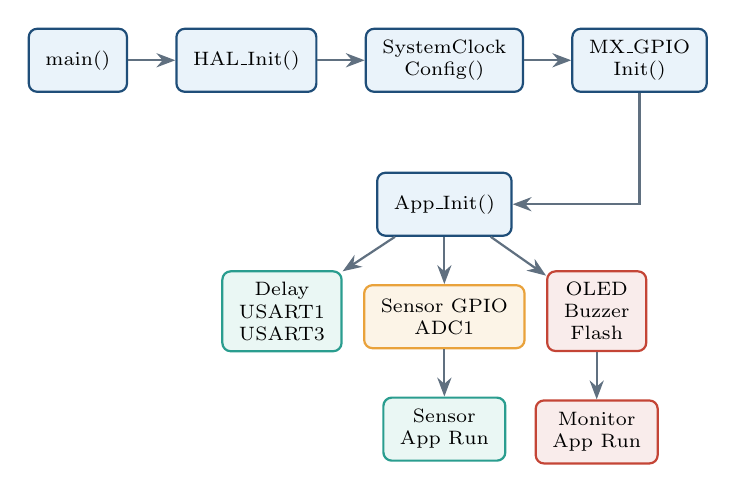
\begin{tikzpicture}[node distance=6mm, font=\scriptsize]
    \node[nodebox] (main) {main()};
    \node[nodebox, right=of main] (hal) {HAL\_Init()};
    \node[nodebox, right=of hal] (clk) {SystemClock\\Config()};
    \node[nodebox, right=of clk] (gpio) {MX\_GPIO\\Init()};
    \node[nodebox, below=10mm of clk] (app) {App\_Init()};
    \node[greenbox, below left=of app] (common) {Delay\\USART1\\USART3};
    \node[amberbox, below=of app] (sensor) {Sensor GPIO\\ADC1};
    \node[redbox, below right=of app] (monitor) {OLED\\Buzzer\\Flash};
    \node[greenbox, below=of sensor] (sloop) {Sensor\\App Run};
    \node[redbox, below=of monitor] (mloop) {Monitor\\App Run};

    \draw[arrow] (main) -- (hal);
    \draw[arrow] (hal) -- (clk);
    \draw[arrow] (clk) -- (gpio);
    \draw[arrow] (gpio) |- (app);
    \draw[arrow] (app) -- (common);
    \draw[arrow] (app) -- (sensor);
    \draw[arrow] (app) -- (monitor);
    \draw[arrow] (sensor) -- (sloop);
    \draw[arrow] (monitor) -- (mloop);
  \end{tikzpicture}
  \vspace{0.5em}
  \small 公共外设先初始化，角色专属外设后初始化，逻辑分层清晰，便于定位问题。
\end{frame}

\begin{frame}{板 A 采集节点主循环 / Sensor Super-Loop}
  \centering
  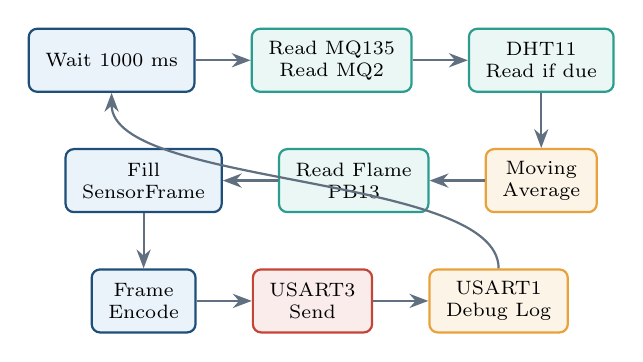
\begin{tikzpicture}[node distance=7mm, font=\scriptsize]
    \node[nodebox] (wait) {Wait 1000 ms};
    \node[greenbox, right=of wait] (adc) {Read MQ135\\Read MQ2};
    \node[greenbox, right=of adc] (dht) {DHT11\\Read if due};
    \node[amberbox, below=of dht] (avg) {Moving\\Average};
    \node[greenbox, left=of avg] (flame) {Read Flame\\PB13};
    \node[nodebox, left=of flame] (frame) {Fill\\SensorFrame};
    \node[nodebox, below=of frame] (encode) {Frame\\Encode};
    \node[redbox, right=of encode] (send) {USART3\\Send};
    \node[amberbox, right=of send] (log) {USART1\\Debug Log};

    \draw[arrow] (wait) -- (adc);
    \draw[arrow] (adc) -- (dht);
    \draw[arrow] (dht) -- (avg);
    \draw[arrow] (avg) -- (flame);
    \draw[arrow] (flame) -- (frame);
    \draw[arrow] (frame) -- (encode);
    \draw[arrow] (encode) -- (send);
    \draw[arrow] (send) -- (log);
    \draw[arrow] (log.north) .. controls +(0,1.2) and +(0,-1.2) .. (wait.south);
  \end{tikzpicture}
  \vspace{0.5em}
  \begin{block}{设计重点}
    每秒发帧，不阻塞显示端；MQ 每帧采样并做整数滑动平均，DHT11 按 $>$2s 间隔刷新，错误通过状态位上报。
  \end{block}
\end{frame}

\begin{frame}{DHT11 单总线时序 / DHT11 Timing}
  \begin{columns}[T,onlytextwidth]
    \begin{column}{0.55\textwidth}
      \begin{enumerate}
        \item MCU 将 PB12 配成开漏输出。
        \item 拉低数据线约 20 ms 发起读取。
        \item 释放数据线，切换为输入。
        \item 等待 DHT11 响应低/高/低脉冲。
        \item 读取 40 bit 数据并校验。
      \end{enumerate}
    \end{column}
    \begin{column}{0.42\textwidth}
      \begin{block}{函数拆分}
        \begin{itemize}
          \item \code{DHT11_SetOutput()}
          \item \code{DHT11_SetInput()}
          \item \code{DHT11_WaitLevel()}
          \item \code{DHT11_Read()}
        \end{itemize}
      \end{block}
    \end{column}
  \end{columns}
  \vspace{0.4em}
  \begin{alertblock}{鲁棒性}
    DHT11 失败不会卡死系统，而是设置 \code{STATUS_DHT_ERROR}，让板 B 显示预警状态。
  \end{alertblock}
\end{frame}

\begin{frame}{MQ 传感器采样与滤波 / ADC And Filtering}
  \begin{columns}[T,onlytextwidth]
    \begin{column}{0.48\textwidth}
      \begin{block}{ADC 通道}
        \begin{itemize}
          \item MQ135 AO：PA4 / ADC1\_CH4
          \item MQ2 AO：PA5 / ADC1\_CH5
          \item ADC1 时钟：72 MHz / 6 = 12 MHz
        \end{itemize}
      \end{block}
    \end{column}
    \begin{column}{0.48\textwidth}
      \begin{block}{指数滑动平均}
        \[
          avg_{new} = \frac{3 \times avg_{old} + raw}{4}
        \]
        \begin{itemize}
          \item 不保存数组窗口。
          \item 计算量小，适合 STM32F103。
          \item 平滑噪声但保留变化趋势。
        \end{itemize}
      \end{block}
    \end{column}
  \end{columns}
\end{frame}

\begin{frame}{串口数据帧协议 / USART3 Frame Protocol}
  \small
  \begin{tabularx}{\textwidth}{@{}p{0.10\textwidth}p{0.18\textwidth}Y@{}}
    \toprule
    Index & Field & Meaning \\
    \midrule
    0--1 & \code{AA 55} & Frame header, used for resynchronization \\
    2 & \code{LEN} & Payload length, fixed to 9 \\
    3--4 & \code{TEMP/HUMI} & DHT11 temperature and humidity \\
    5--8 & \code{MQ135/MQ2} & ADC readings, high byte first \\
    9 & \code{FLAME} & 1 means flame detected \\
    10 & \code{SEQ} & Rolling frame number \\
    11 & \code{STATUS} & bit0 = DHT11 error \\
    12 & \code{CHECKSUM} & Low 8 bits of LEN + payload \\
    \bottomrule
  \end{tabularx}
  \vspace{0.4em}
  \begin{block}{核心函数}
    \code{Frame_Encode()} 负责结构体转字节帧，\code{Frame_Decode()} 负责帧头、长度、校验和验证。
  \end{block}
\end{frame}

\begin{frame}{板 B 接收设计 / Interrupt + Ring Buffer}
  \centering
  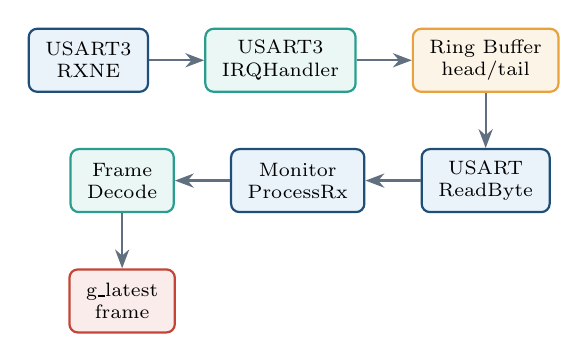
\begin{tikzpicture}[node distance=7mm, font=\scriptsize]
    \node[nodebox] (rx) {USART3\\RXNE};
    \node[greenbox, right=of rx] (isr) {USART3\\IRQHandler};
    \node[amberbox, right=of isr] (buf) {Ring Buffer\\head/tail};
    \node[nodebox, below=of buf] (read) {USART\\ReadByte};
    \node[nodebox, left=of read] (parse) {Monitor\\ProcessRx};
    \node[greenbox, left=of parse] (decode) {Frame\\Decode};
    \node[redbox, below=of decode] (state) {g\_latest\\frame};

    \draw[arrow] (rx) -- (isr);
    \draw[arrow] (isr) -- (buf);
    \draw[arrow] (buf) -- (read);
    \draw[arrow] (read) -- (parse);
    \draw[arrow] (parse) -- (decode);
    \draw[arrow] (decode) -- (state);
  \end{tikzpicture}
  \vspace{0.5em}
  \begin{block}{为什么这样设计}
    中断只收字节，主循环解析完整帧。这样 ISR 短小稳定，OLED 刷新时也不容易漏掉串口数据。
  \end{block}
\end{frame}

\begin{frame}{板 B 协作式调度 / Monitor Scheduler}
  \begin{tabularx}{\textwidth}{@{}p{0.22\textwidth}p{0.18\textwidth}Y@{}}
    \toprule
    任务 & 周期 & 函数与作用 \\
    \midrule
    串口解析 & 每轮循环 & \code{Monitor_ProcessRx()}，尽快消化接收缓冲 \\
    按键扫描 & 每轮循环 & \code{Monitor_UpdateButtons()}，保证 K1/K2 响应 \\
    报警输出 & 100 ms & \code{Monitor_UpdateAlarm()}，更新 LED 和蜂鸣节奏 \\
    OLED 刷新 & 300 ms & \code{Monitor_UpdateDisplay()}，控制刷新负担 \\
    Flash 记录 & 10 s & \code{Flash_LogFrame()}，降低写入频率 \\
    \bottomrule
  \end{tabularx}
  \vspace{0.5em}
  \begin{block}{无 RTOS 的处理方式}
    使用 \code{HAL_GetTick()} 做时间片调度，避免长阻塞，让串口、显示、按键、报警共存。
  \end{block}
\end{frame}

\begin{frame}{报警状态机 / Alarm State Machine}
  \centering
  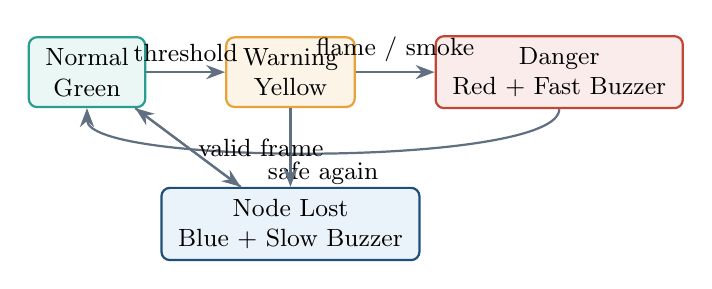
\begin{tikzpicture}[node distance=10mm, font=\small]
    \node[greenbox] (normal) {Normal\\Green};
    \node[amberbox, right=of normal] (warn) {Warning\\Yellow};
    \node[redbox, right=of warn] (danger) {Danger\\Red + Fast Buzzer};
    \node[nodebox, below=of warn] (lost) {Node Lost\\Blue + Slow Buzzer};

    \draw[arrow] (normal) -- node[above]{threshold} (warn);
    \draw[arrow] (warn) -- node[above]{flame / smoke} (danger);
    \draw[arrow] (danger) .. controls +(0,-1.2) and +(0,-1.2) .. node[below]{safe again} (normal);
    \draw[arrow] (normal) -- (lost);
    \draw[arrow] (warn) -- (lost);
    \draw[arrow] (lost) -- node[right]{valid frame} (normal);
  \end{tikzpicture}
  \vspace{0.5em}
  \small 优先级：Danger > Node Lost > Warning > Normal。静音只影响蜂鸣器，不改变 LED 状态。
\end{frame}

\begin{frame}{OLED 页面设计 / OLED UI}
  \begin{columns}[T,onlytextwidth]
    \begin{column}{0.47\textwidth}
      \begin{block}{Page 0：监测页}
        \begin{itemize}
          \item 系统状态：NORMAL / WARN / DANGER / NODE LOST
          \item 温度、湿度
          \item MQ135 空气质量 ADC
          \item MQ2 烟雾 ADC 与火焰状态
        \end{itemize}
      \end{block}
    \end{column}
    \begin{column}{0.47\textwidth}
      \begin{block}{Page 1：参数页}
        \begin{itemize}
          \item 当前阈值档位
          \item 空气质量预警阈值
          \item 烟雾预警/危险阈值
          \item 帧序号与 Flash 状态
        \end{itemize}
      \end{block}
    \end{column}
  \end{columns}
  \vspace{0.4em}
  \small K1 切换页面，K2 短按静音，K2 长按切换阈值档位。
\end{frame}

\begin{frame}{OLED 驱动分层 / OLED Driver Stack}
  \centering
  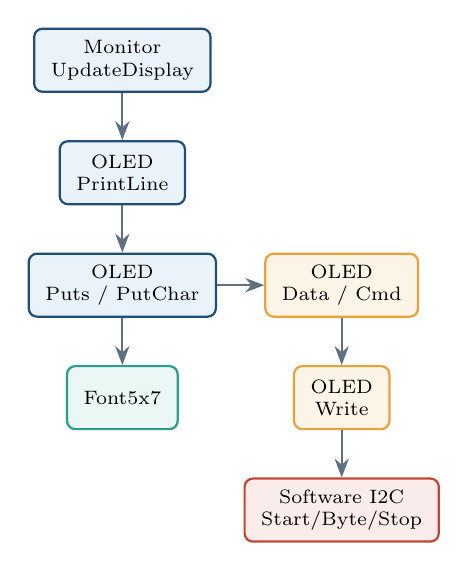
\begin{tikzpicture}[node distance=6mm, font=\scriptsize]
    \node[nodebox] (page) {Monitor\\UpdateDisplay};
    \node[nodebox, below=of page] (line) {OLED\\PrintLine};
    \node[nodebox, below=of line] (text) {OLED\\Puts / PutChar};
    \node[greenbox, below=of text] (font) {Font5x7};
    \node[amberbox, right=of text] (data) {OLED\\Data / Cmd};
    \node[amberbox, below=of data] (write) {OLED\\Write};
    \node[redbox, below=of write] (i2c) {Software I2C\\Start/Byte/Stop};

    \draw[arrow] (page) -- (line);
    \draw[arrow] (line) -- (text);
    \draw[arrow] (text) -- (font);
    \draw[arrow] (text) -- (data);
    \draw[arrow] (data) -- (write);
    \draw[arrow] (write) -- (i2c);
  \end{tikzpicture}
\end{frame}

\begin{frame}{按键交互 / Button Interaction}
  \begin{tabularx}{\textwidth}{@{}p{0.18\textwidth}p{0.30\textwidth}Y@{}}
    \toprule
    按键 & 操作 & 系统反馈 \\
    \midrule
    K1 & 短按 & \code{g_page} 翻转，OLED 在监测页与参数页之间切换 \\
    K2 & 短按 & \code{g_mute_until_ms = now + 60000}，蜂鸣器静音 60 秒 \\
    K2 & 长按 & \code{g_threshold_profile} 递增，切换阈值档位 \\
    \bottomrule
  \end{tabularx}
  \vspace{0.5em}
  \begin{block}{边沿检测}
    使用 \code{k1_last}、\code{k2_last} 保存上一次电平，只在按下或松开边沿触发动作，避免按住时重复执行。
  \end{block}
\end{frame}

\begin{frame}{可选 Flash 记录 / Optional W25Q64 Logging}
  \begin{columns}[T,onlytextwidth]
    \begin{column}{0.53\textwidth}
      \begin{block}{初始化策略}
        \begin{itemize}
          \item SPI2 使用 PB13/PB14/PB15。
          \item PB12 作为 CS。
          \item 读取 JEDEC ID 判断芯片是否存在。
          \item 未检测到芯片时主流程继续运行。
        \end{itemize}
      \end{block}
    \end{column}
    \begin{column}{0.43\textwidth}
      \begin{block}{记录内容}
        \begin{itemize}
          \item 帧序号与状态位
          \item 温湿度、MQ ADC、火焰状态
          \item 当前报警状态
          \item \code{HAL_GetTick()} 时间戳
          \item 阈值档位与 checksum
        \end{itemize}
      \end{block}
    \end{column}
  \end{columns}
\end{frame}

\begin{frame}{关键全局状态 / Shared State Variables}
  \scriptsize
  \begin{tabularx}{\textwidth}{@{}p{0.22\textwidth}p{0.24\textwidth}Y@{}}
    \toprule
    变量 & 写入者 & 读取者与作用 \\
    \midrule
    \code{g_latest_frame} & \code{Monitor_ProcessRx()} & OLED、报警、Flash 使用的最新合法数据 \\
    \code{g_last_rx_ms} & \code{Monitor_ProcessRx()} & \code{Monitor_NodeLost()} 判断离线 \\
    \code{g_page} & \code{Monitor_UpdateButtons()} & OLED 页面选择 \\
    \code{g_threshold_profile} & \code{Monitor_UpdateButtons()} & 影响报警阈值与显示参数 \\
    \code{g_mute_until_ms} & \code{Monitor_UpdateButtons()} & 控制蜂鸣器静音截止时间 \\
    \code{g_flash_present} & \code{Flash_Init_Custom()} & 控制是否启用日志记录 \\
    \code{rx_buf/head/tail} & ISR / parser & USART3 接收环形缓冲区，负责中断与主循环之间的数据交接 \\
    \bottomrule
  \end{tabularx}
\end{frame}

\begin{frame}{端到端数据路径 / End-to-End Data Path}
  \centering
  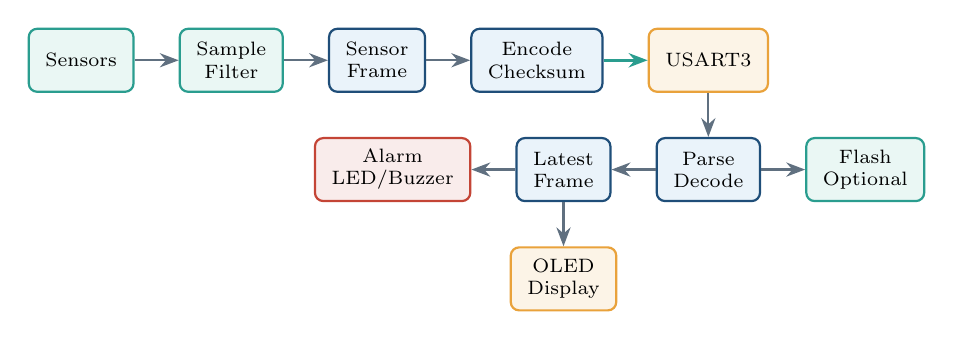
\begin{tikzpicture}[node distance=5.6mm, font=\scriptsize]
    \node[greenbox] (sensors) {Sensors};
    \node[greenbox, right=of sensors] (sample) {Sample\\Filter};
    \node[nodebox, right=of sample] (frame) {Sensor\\Frame};
    \node[nodebox, right=of frame] (encode) {Encode\\Checksum};
    \node[amberbox, right=of encode] (uart) {USART3};
    \node[nodebox, below=of uart] (parse) {Parse\\Decode};
    \node[nodebox, left=of parse] (state) {Latest\\Frame};
    \node[redbox, left=of state] (alarm) {Alarm\\LED/Buzzer};
    \node[amberbox, below=of state] (oled) {OLED\\Display};
    \node[greenbox, right=of parse] (flash) {Flash\\Optional};

    \draw[arrow] (sensors) -- (sample);
    \draw[arrow] (sample) -- (frame);
    \draw[arrow] (frame) -- (encode);
    \draw[bus] (encode) -- (uart);
    \draw[arrow] (uart) -- (parse);
    \draw[arrow] (parse) -- (state);
    \draw[arrow] (state) -- (alarm);
    \draw[arrow] (state) -- (oled);
    \draw[arrow] (parse) -- (flash);
  \end{tikzpicture}
\end{frame}

\begin{frame}{异常处理 / Fault Handling}
  \small
  \begin{tabularx}{\textwidth}{@{}p{0.25\textwidth}p{0.30\textwidth}Y@{}}
    \toprule
    异常 & 检测位置 & 处理方式 \\
    \midrule
    DHT11 读取失败 & \code{DHT11_Read()} & 设置 \code{STATUS_DHT_ERROR}，继续发帧 \\
    串口噪声或错位 & \code{Frame_Decode()} & 丢弃坏帧，重新寻找 \code{AA 55} \\
    接收缓冲满 & \code{USART3_IRQHandler()} & 丢弃最新字节，避免 ISR 阻塞 \\
    板 A 离线 & \code{Monitor_NodeLost()} & OLED 显示 NODE LOST，蓝灯慢蜂鸣 \\
    Flash 未接入 & \code{Flash_Init_Custom()} & \code{g_flash_present=0}，主功能不受影响 \\
    时钟初始化失败 & \code{SystemClock_Config()} & \code{Error_Handler()} 停机保护 \\
    \bottomrule
  \end{tabularx}
\end{frame}

\begin{frame}{测试计划 / Test Plan}
  \begin{columns}[T,onlytextwidth]
    \begin{column}{0.5\textwidth}
      \begin{block}{单节点测试}
        \begin{itemize}
          \item 板 A：DHT11、MQ135、MQ2、火焰模块。
          \item 板 B：OLED、RGB、蜂鸣器、K1/K2。
          \item USART1 日志：\code{115200 8N1}。
        \end{itemize}
      \end{block}
    \end{column}
    \begin{column}{0.46\textwidth}
      \begin{block}{系统测试}
        \begin{itemize}
          \item USART3 双板通信。
          \item 断线后 \code{NODE LOST}。
          \item 烟雾/火焰触发报警。
          \item 任意节点重启恢复。
        \end{itemize}
      \end{block}
    \end{column}
  \end{columns}
\end{frame}

\begin{frame}{演示流程 / Demonstration Flow}
  \begin{enumerate}
    \item 烧录 \code{Fire_F103_sensor.hex} 到板 A，烧录 \code{Fire_F103_monitor.hex} 到板 B。
    \item 连接 USART3：A PB10 到 B PB11，B PB10 到 A PB11，并共地。
    \item 打开两个 CH340C 串口，确认板 A \code{[SENSOR]} 日志和板 B \code{[MONITOR] rx} 日志。
    \item 展示 OLED 监测页和参数页，按 K1 切换页面。
    \item 触发烟雾/火焰模块，观察状态灯和蜂鸣器变化。
    \item 短按 K2 展示静音，长按 K2 展示阈值档位切换。
    \item 断开 USART3，展示 \code{NODE LOST} 自动检测。
  \end{enumerate}
\end{frame}

\begin{frame}[fragile]{构建与仓库结构 / Build And Repository}
  \begin{columns}[T,onlytextwidth]
    \begin{column}{0.48\textwidth}
\begin{lstlisting}[style=cstyle]
cmake --preset SensorDebug
cmake --build --preset SensorDebug

cmake --preset MonitorDebug
cmake --build --preset MonitorDebug
\end{lstlisting}
    \end{column}
    \begin{column}{0.48\textwidth}
      \begin{block}{文档结构}
        \begin{itemize}
          \item \code{README.md} / \code{README.zh-CN.md}
          \item \code{WIRING.md}
          \item \code{docs/FUNCTION_GUIDE.md}
          \item \code{docs/FUNCTION_DESIGN_WALKTHROUGH.*.md}
          \item \code{docs/PROJECT_STRUCTURE.md}
        \end{itemize}
      \end{block}
    \end{column}
  \end{columns}
\end{frame}

\begin{frame}{当前限制 / Current Limitations}
  \begin{tabularx}{\textwidth}{@{}p{0.30\textwidth}Y@{}}
    \toprule
    限制 & 说明 \\
    \midrule
    MQ 数值未标定 ppm & 当前使用原始 ADC 值，需要实测标定曲线才能换算浓度 \\
    通信仍以单向上报为主 & 预留了 B 到 A 的 ACK/心跳方向，但基础版本先保证 A 到 B 稳定 \\
    OLED 文本较简单 & 为保证 0.96 寸屏幕可读性，使用 4 行英文/数字状态文本 \\
    Flash 记录为演示型 & 使用第 0 扇区循环写，不是工业级 wear leveling \\
    \bottomrule
  \end{tabularx}
\end{frame}

\begin{frame}{可扩展方向 / Future Work}
  \begin{columns}[T,onlytextwidth]
    \begin{column}{0.5\textwidth}
      \begin{block}{功能扩展}
        \begin{itemize}
          \item B 到 A ACK / 心跳。
          \item 阈值写入 W25Q64，重启保持。
          \item 增加光敏、人体红外等传感器。
          \item 历史记录导出到 PC。
        \end{itemize}
      \end{block}
    \end{column}
    \begin{column}{0.46\textwidth}
      \begin{block}{工程改进}
        \begin{itemize}
          \item 拆分 \code{main.c} 为 protocol、sensor、monitor 模块。
          \item 增加 CRC8/CRC16。
          \item 更完整的按键消抖。
          \item 增加单元测试或串口帧模拟器。
        \end{itemize}
      \end{block}
    \end{column}
  \end{columns}
\end{frame}

\begin{frame}{总结 / Summary}
  \begin{block}{项目成果}
    本系统完成了双 STM32 节点分工、USART3 数据通信、本地 OLED 显示、RGB/蜂鸣器报警、按键交互和可选 Flash 记录。
  \end{block}
  \begin{block}{工程价值}
    项目体现了嵌入式系统中的资源规划、通信协议设计、状态机、协作式调度和异常恢复思路。
  \end{block}
  \begin{center}
    \Large 谢谢观看 / Thank you
  \end{center}
\end{frame}

\end{document}
